\title{LEZIONE 9 28/04/2020}\newline
\textbf{link} \href{https://web.microsoftstream.com/video/673607e9-751d-488b-bb1d-79ee783a9b29}{clicca qui}
\section{Dinamica}
Esistono diverse modalità per studiare la dinamica di un sistema meccanico:
\begin{itemize}
    \item \textbf{Equilibri dinamici}:
    \begin{itemize}
        \item \textbf{Principio di D'Alambert}
        \item \textbf{Equazioni cardinali della statica}
    \end{itemize}
    \item \textbf{Approcci energetici}:
    \begin{itemize}
        \item \textbf{Principio dei Lavori Virtuali (PLV)}
        \item \textbf{Bilancio di Potenze (BdP)} o \textbf{Teroema dell'energia cinetica}
        \item \textbf{Equazioni di Lagrange}
    \end{itemize}
\end{itemize}
\newpage
\section{Principio di D'Alambert}
Il principio di D'Alambert si basa sulla scrittura di equazioni di equilibrio dinamico.\newline
\newline
Secondo questo approccio la dinamica viene studiata come una condizione statica equivalente. In poche parole andremmo a generalizzare le equazioni cardinali della statica, andando ad aggiungere tra le forze che agiscono sul punto o sui corpi rigidi anche le forze e coppie di inerzia che agiscono sul sistema stesso.
\subsection{Principio di D'Alament per il punto materiale}
Partiamo dal secondo principio della dinamica o \textbf{prima legge di Newton}:\newline
Se abbiamo un punto materiale di massa $m$, che si muove con una certa accellerazione $a$ e sul quale agiscono un certo numero di forze $\vec{F}_1, \vec{F}_2, \dots, \vec{F}_i$, la risultante delle forze sul punto dovrà eguagliare il prodotto fra la massa del punto e l'accellerazione del punto (\textbf{forza = massa x accellerazione}):
\[
    \sum_{i} \vec{F}_{i} = m \cdot \vec{a}
\]
\ \newline
Se ora andiamo a definire una quantità $\vec{F}_{in}$, detta \textbf{forza di inerzia}, che è pari al prodotto fra la massa e l'accellerazione del punto cambiata di segno
\[
    \vec{F}_{in} = - m \cdot  \vec{a}
\]
allora possiamo riscrivere la legge di Newton come:
\[
    \sum_{i} \vec{F}_i - m \vec{a} = \sum_{i} \vec{F}_{i} + \vec{F}_{in}
\]
Quindi introducendo questa forza di inerzia ora posso studiare la dinamica di un corpo come un'equilibrio (dinamico) della prima legge di Newton.\newline
\newline
\textbf{Principio di D'Alambert per il punto materiale}:
\[
    \sum_{i} \vec{F}_{i} + \vec{F}_{in} = 0
\]
Il principio di D'Alambert altro non è che l'annullamento di tutte le forze agenti sul punto materiale, incluse le forze di inerzia, cioè le forze che rappresentano la resistenza di un punto nel mettersi in moto.\newline
\newline
Condizione sufficiente e necessaria per l'equilibrio dinamico di un punto è che si annulli la risultante di tutte le forze, attive e reattive, applicate sul punto stesso, incluse le forze d'inerzia.\newline
\newline
Facendo così il problema dinamico viene ricondotto a un problema statico.\newline
\newline
L'equazione di equilibrio del principio di D'alambert è un'equazione vettoriale, che quindi nel piano può essere proiettato sugli assi in modo da ottenere un sistema in due equazioni linearmente indipendenti che ci permettono:
\begin{itemize}
    \item di calcolare le reazioni vincolari;
    \item se sono note le forze attive applicate al punto, di determinare il moto del punto, ovvero velocità e accellerazioni;
    \item se è noto il moto del punto, ovvero velocità e accellerazione, di calcolare le forze attive necessarie per mantenere la condizione di moto assegnata.
\end{itemize}
\subsection{Principio di D'Alambert per il corpo rigido: forze e coppie di inerzia}
Valgono le stesse considerazioni fatte per il punto materiale: si estendono le equazioni cardinali della statica, aggiungendo le forze di inerzia che agiscono sul corpo rigido.\newline
\newline
\textbf{Principio di D'Alambert per il corpo rigido}:\newline
Condizione necessaria e sufficiente per l'equilibrio dinamico di un corpo rigido è che si annulli la risultante e il momento risultante rispetto a un generico polo $O$ di tutte le forze e coppie esterne, attive e reattive, agenti su di esso, incluse le forze e coppie di inerzia.\newline
\newline
Definiamo quindi \textbf{forze e coppie di inerzia} per un copro rigido:\newline
[immagine dagli appunti del prof]
\begin{center}
    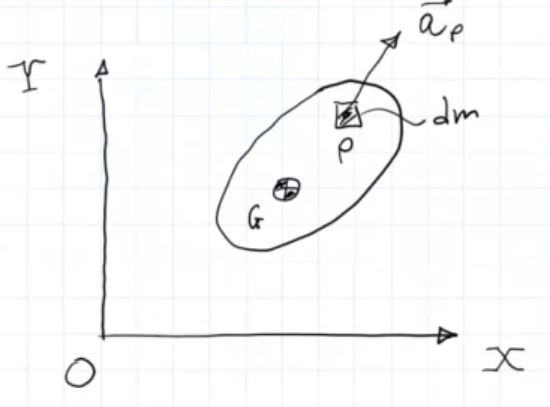
\includegraphics[height=3cm]{../lezione9/img1.JPG}
\end{center}
Dato una sezione infinitesima $P$ del corpo rigido, con massa $dm$ e accellerazione $\vec{a}_P$, allora $d \vec{F}_{in} = - \vec{a}_P \cdot dm$, inoltre, siccome $dm = \rho dV$, allora $d \vec{F}_{in} = - \vec{a}_P \rho dV$.
\subsection*{Forza di inerzia}
Ora per trovare la \textbf{forza di inerzia del corpo rigido} è sufficiente estendere la formula con l'integrale su tutta la superficie del corpo:
\[
    \vec{F}_{in} = - \int_V \vec{a}_P \rho dV
\]
Per risolvere questo integrale usiamo il teorema di Rivals applicato rispetto al barcentro $G$ del corpo per determinare l'acellerazione del genrico punto $P$: $\vec{a}_P = \vec{a}_G + \dot{\vec{\omega}}\land(P-G) + \vec{\omega}\land [\vec{\omega}\land (P-G)]$.\newline
L'accellerazione del punto $P$ è vista come la somma dell'accellerazione del baricentro  $\vec{a}_G$  e  dell'accellerazione del punto $P$ rispetto a $G$ mentre il corpo ruota attorno ad un asse $z$ perpendicolare al piano del foglio e passante per il punto $G$, che essendo un moto rotatorio è composto da due componenti, una tangenziale $a_{PG}^{(t)} = \dot{\vec{\omega}}\land(P-G)$ e una normale $a_{PG}^{(n)}\vec{\omega}\land [\vec{\omega}\land (P-G)]$.\newline
Sostituendo ora l'accellerazione del $\vec{a}_P$ nell'integrale otteniamo:
\[
    \vec{F}_{in} = - \int_V \vec{a}_G \rho dV - \int_V \left[ \dot{\vec{\omega}} \land (P-G) \right] \rho dV - \int_V \left[ \vec{\omega} \land (\vec{\omega} \land (P-G)) \right] \rho dV
\]
\[
    \vec{F}_{in} = - \vec{a}_G \int_V \rho d V - \dot{\vec{\omega}} \land \int_V (P-G) \rho dV - \vec{\omega} \land \vec{\omega} \land \int_V (P-G) \rho dV
\]
Analiziamo quindi ora il termine $\int_V (P-G) \rho dV$:\newline[immagine dagli appunti del prof]
\begin{center}
    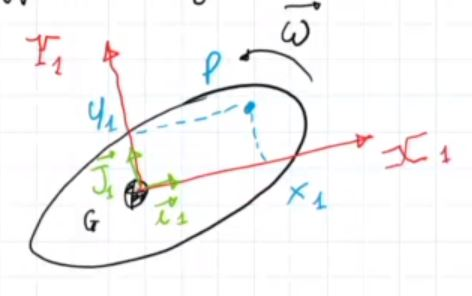
\includegraphics[height=3cm]{../lezione9/img2.JPG}
\end{center}
Considerando un sistema di riferimento che ha origine nel baricentro possiamo scrivere il vettore $(P-G) = X_1 \vec{i}_1 + Y_1 \vec{j}_1$, per cui possiamo svolgere l'integrale come
\[
    \int_V (P-G) \rho dV = \vec{i}_1 \int_V X_1 \rho dV + \vec{j}_1 \int_V Y_1 \rho dV
\]
dove il temine $\vec{i}_1 \int_V X_1 \rho dV = S_y$ è il momento statico del prim'ordine rispetto all'asse $Y$ di un sistema di riferimento che ha origine nel baricentro, analogamente il termine $\vec{j}_1 \int_V Y_1 \rho dV = S_x$ è il momento statico del prim'ordine rispetto all'asse $X$. Per definizione i momenti statici rispetto a un baricentro sono nulli, quindi l'integrale $\int_V (P-G) \rho dV$ è nullo.\newline
\newline
Quindi tutto ciò che rimane nella definizione della \textbf{forza di inerzia} è:
\[
    \vec{F}_{in} = - \vec{a}_G \int_V \rho dV = - m \vec{a}_G
\]
dove $\int_V \rho dV = m$.\newline
\newline
Quindi la forza di inerzia di un corpo rigido è la sua massa moltiplicata per l'accellerazione del baricentro. Notiamo come ancora una volta il baricentro può essere visto come quel punto in cui è concentrata tutta la massa del corpo.
\subsection*{Coppia di inerzia}
Bisogna calcolare il momento risultante di tutte le forze di inerzia infinitesime rispetto al baricentro del corpo
\[
    \vec{C}_{in} = \int_V (P-G) \land d \vec{F}_{in} =  - \int_V (P-G) \land \vec{a}_P \rho dV
\]
e con dei passaggi del tutto analoghi a quelli precedenti, cioè passando per il teorema di Rivals otteniamo l'accellerazione del punto $P$: $\vec{a}_P = \vec{a}_G + \dot{\vec{\omega}} \land (P-G) + \vec{\omega} \land \vec{\omega} \land (P-G)$ e quindi otteniamo che
\[
    (P-G) \land \vec{a}_P = (P-G) \land \vec{a}_G + (P-G) \land \dot{\vec{\omega}} \land (P-G) + \cancel{(P-G) \land \vec{\omega} \land \vec{\omega} \land (P-G)}
\]
\ \newline
Il termine accellerazione normale $ \vec{a}_{PG}^{(n)} \vec{\omega} \land \vec{\omega} \land (P-G)$ è parallelo al vettore $(P-G)$ e il prodotto vettoriale fra due vettori paralleli è nullo, quindi l'ultimo termine è nullo.\newline
\newline
Analiziamo ora il termine $(P-G) \land \dot{\vec{\omega}} \land (P-G)$.\newline
[immagine dagli appunti del prof]
\begin{center}
    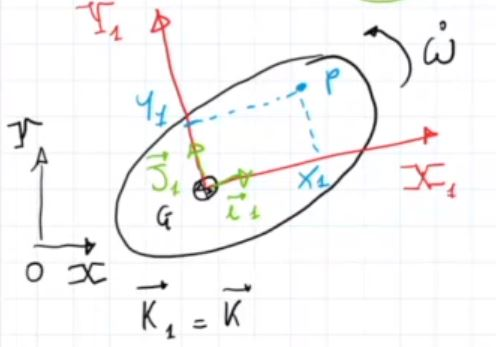
\includegraphics[height=3cm]{../lezione9/img3.JPG}
\end{center}
\[
    (P-G) \land \dot{\vec{\omega}} \land (P-G) = (x_1 \vec{i}_1 + y_1 \vec{j}_1) \land \left[ \dot{\omega} \vec{k} \land (x_1 \vec{i}_1 + y_1 \vec{j}_1) \right] =
\]
\[
    =  (x_1 \vec{i}_1 + y_1 \vec{j}_1) \land \left[ \dot{\omega} x_1 \vec{j}_1 - \dot{\omega} y_1 \vec{i}_1 \right] = \dot{\omega} x_1^2 \vec{k} + \dot{\omega} y_1^2 \vec{k}
\]
\[
    = \dot{\omega} \vec{k} (x_1^2 + y_1^2) = \dot{\vec{\omega}} \bar{PG}^2
\]
\ \newline
Sostituendo ora tutto all'interno della definizione iniziale di coppia di inerzia otteniamo:
\[
    C_{in} = - \int_V (P-G) \land \vec{a}_P rho dV = - \left[\int_V (P-G) \rho dV\right] \land \vec{a}_G - \dot{\vec{\omega}} \int_V (x_1^2 + y_1^2) \rho dV 
\]
Per quello che abbiamo detto prima sulle forze di inerzia, il termine $\left[\int_V (P-G) \rho dV\right]$ è nullo.\newline
Sul secondo termine sappiamo che $(x_1^2 + y_1^2) = \bar{PG}^2$ è la distanza al quadrato del punto $P$ dal baricentro, quindi il temrine $\int_V (x_1^2 + y_1^2) \rho dV $ non è altro che il \textbf{momento baricentrico} $J_G$ (visto la scorsa lezione).\newline
\newline
Infine dunque la \textbf{coppia di inerzia} può essere scritta come il prodotto del momento baricentrico per l'accellerazione angolare cambiato di segno:
\[
    \vec{C}_{in} = - J_G \dot{\vec{\omega}}
\]
\subsection*{Principio di D'Alambert}
Vediamo infine i risultati fino ad ora ottenuti applicati al principio di D'Alambert:
\[
    \begin{cases}
        \sum_i \vec{F}_i + \vec{F}_in = 0\\
        \sum_i (P_i - O) \land \vec{F}_i + \sum_j \vec{C}_j - (G-O) \land \vec{F}_{in} + \vec{C}_{in} = 0
    \end{cases}
\]
con $O$ polo scelto arbitrariamente e $P_i$ punto di applicazione della forza $i$-esima.\newline
\newline
Questo sistema di due equazioni, nel piano rappresenta un sistema di tre equazioni linearmente indipendenti che ci permettono:
\begin{itemize}
    \item di calcolare le reazioni vincolari;
    \item se sono note le forze attive applciate al corpo rigido, di determinare tanti parametri cinematici che definiscono il moto del corpo, tanti quanti sono i gradi di libertà del sistema ($3-n_v \geq 1$) (\textbf{dinamica direatta});
    \item se è assegnata la velocità e accellerazione del corpo, di determinare le forze attive necessarie a mantenere le condizioni di moto assegnate (\textbf{dinamica inversa}).
\end{itemize}
\ \newline
\newline
\textbf{es.} dinamica inversa:\newline
[immagine dagli appunti del prof]
\begin{center}
    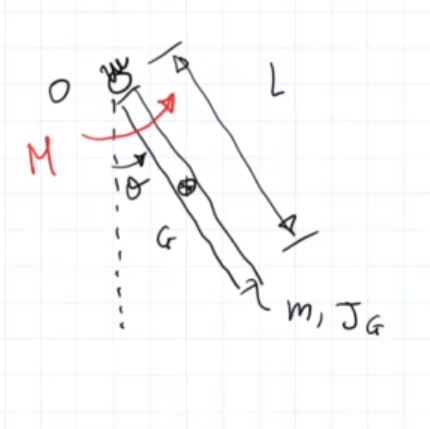
\includegraphics[height=3cm]{../lezione9/img4.JPG}
\end{center}
Dati: $\theta = 30^0$, $\dot{\theta} = 3 rad/s$, $\ddot{\theta} = 1 rad/s^2$, $m = 6 kg$, $L = 1m$, trave snella, omogenea, nel piano verticale.\newline
Problema: trovare il momento angolare $M$ che mi consente di mantenere la condizione di moto assegnata.\newline
\newline
Per prima cosa procediamo con un analisi cinematica del problema per determinare le accellerazioni, che mi consentiranno di determinare le coppie e forze di inerzia.\newline
In seguito isoleremo il corpo per mettere in evidenza tutte le forze attive e reattive.\newline
Come ultima cosa applicheremo il principio di D'Alambert.\newline
\newline
Analisi cinemaitca:\newline
[immagine dagli appunti del prof]
\begin{center}
    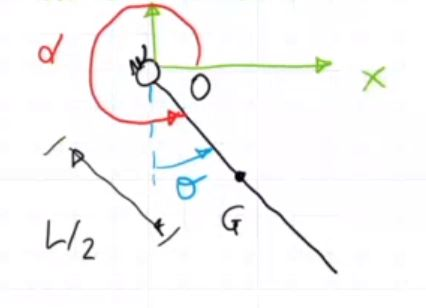
\includegraphics[height=3cm]{../lezione9/img5.JPG}
\end{center}
 $(G-O) = \frac{L}{2}e^{i \alpha}$, con $\alpha = \frac{3}{2} \pi + \theta$, $\dot{\alpha} = \dot{\theta} = \omega$, $\ddot{\alpha} = \ddot{\theta} = \dot{\omega}$.\newline
Velocità: $\vec{v}_G = i \dot{\alpha} \frac{L}{2} e^{i \alpha} = \dot{\alpha} \frac{}{2} e^{i (\alpha + \frac{\pi}{2})} = \dot{\theta} \frac{L}{2} e^{i (\alpha + \frac{\pi}{2})}$.\newline
Accellerazione: $\vec{a}_G = \ddot{\alpha} \frac{L}{2} e^{i (\alpha + \frac{\pi}{2})} - \dot{\alpha}^2 \frac{L}{2} e^{i \alpha} = \ddot{\theta} \frac{L}{2} e^{i (\alpha + \frac{\pi}{2})} - \dot{\theta}^2 \frac{L}{2} e^{i \alpha}$, con $a^{(t)}_G = \ddot{\theta} \frac{L}{2} e^{i (\alpha + \frac{\pi}{2})}$ e $a^{(n)}_G = \dot{\theta}^2 \frac{L}{2} e^{i \alpha}$\newline
[immagine dagli appunti del prof]
\begin{center}
    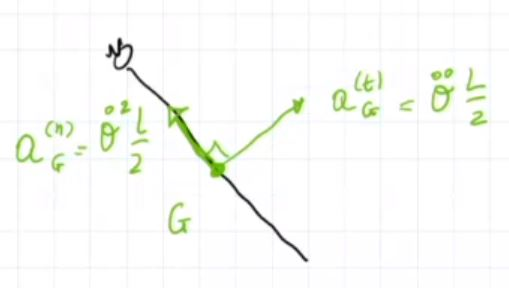
\includegraphics[height=3cm]{../lezione9/img6.JPG}
\end{center}
Possiamo ora calcolare le forze e le coppie d'inerzia:
\[
    \vec{F}_{in} = - m \vec{a}_G = - m (\vec{a}_G^{(t)} + \vec{a}_G^{(n)})
\]
\[
    \vec{C}_{in} = - J_G \dot{\vec{\omega}}
\]
tenendo sempre a mente che $\dot{\omega} = \ddot{\theta}$ e siccome abbiamo una trave snella omogenea, sappiamo che $J_G = \frac{m L^2}{12} = 0,5 kg m^2$.\newline
\newline
A questo punto possiamo isolare il corpo, indicare tutte le forze e scrivere il principio di D'Alambert:\newline
[immagine dagli appunti del prof]
\begin{center}
    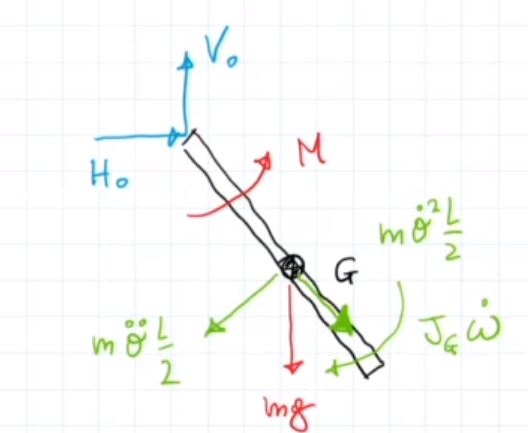
\includegraphics[height=3cm]{../lezione9/img7.JPG}
\end{center}
\[
    \begin{cases}
        R_x = 0\\
        R_y = 0\\
        M_o = 0
    \end{cases} \rightarrow V_o, H_o, M = ?
\]
Calcoliamo il momento ripetto al polo $O$:
\[
    M - mg \frac{L}{2}sin(\theta) - J_G \dot{\omega} - m \ddot{\theta} \frac{L}{2} \frac{L}{2} = 0
\]
\[
    M = \left(J_G + m \frac{L^2}{4}\right) \ddot{\theta} + mg \frac{L}{2} sin(\theta) = 16,7 Nm 
\]
Ora calcoliamo le forze vincolari con gli equilibri sugli assi $X$ e $Y$:
\[
    H_o + m \dot{\theta}^2 \frac{L}{2} sin(\theta) - m \ddot{\theta} \frac{L}{2} cos(\theta) = 0 \Rightarrow H_o = -10,9 N
\]
\[
    V_o - mg - m \frac{L}{2} \ddot{\theta} sin(\theta) - m \frac{L}{2}\dot{\theta}^2 cos(\theta) = 0 \Rightarrow V_o = 83,7N
\]
\rule{\textwidth}{0,4pt}
\subsection{Principio di D'Alambert per sistemi di corpi rigidi}
Come per la statica, ci basta spezzare il sistema in tutti i corpi rigidi che lo costituiscono e verificare le condizioni di equilibrio dinamico per ciascuno di essi.\newline
\newline
\textbf{Principio di D'Alambert per sistemi di corpi rigidi}:\newline
Condizione necessaria e sufficiente per l'equilibrio dinamico di un sistema di corpi rigidi è che sia in equilibrio ogni sua parte supposta rigida sotto l'azione di tutte le forze interne ed esterne, attive e reattive, applicate al corpo, incluse pure le forze e coppie di inerzia.\newline
\newline
Le equazioni del principio di D'Alambert applicato ai sistemi di corpi rigidi ci permettono:
\begin{itemize}
    \item di calcolare le reazioni vincolari;
    \item se sono date le forze attive esterne, di determinare il moto del sistema, ovvero tanti parametri cinematici del sistema, tanti quanti sono i gradi di libertà $n$ del sistema (\textbf{dinamica diretta});
    \item se è assegnata una condizione di moto, di calcolare tante forze necessarie a mantenere la condizione di moto, quanti sono i gradi di libertà del sistema (\textbf{dinamica inversa}).
\end{itemize}